\section{Procedures for detecting and mitigating batch effects}
\label{app:causal_procedures}

\subsection{Detecting batch effects with \ccdcorr}
Many of the more direct types of detectable effects, such as associational and conditional effects, fail to adaequately account for confounding biases present in the data. {\edits{We instead propose the use of \ccdcorr, in which a conditional $K$-sample test \cite{Wang2015} is performed on samples with the same ``range'' of covariate values after propensity trimming via a strategy known as vector matching \cite{Lopez2014}. This strategy is the focus of a complementary theoretical manuscript, in which we illustrate the theoretical and empirical (via simulations) benefits of this technique over competing approaches for detecting causal effects between potential outcomes. This strategy maintains both high sensitivity and specificity under traditionally problematic data regimes (high-dimensionality, non-monotonicities, and non-linearities) in which other methods typically fail \cite{Bridgeford2023Jul}, making it a natural choice for causal discrepancy testing (of which ``batch effect'' detection, termed \textit{causal unconditional discrepancy testing} in \cite{Bridgeford2023Jul}, as-defined herein is a special case).

{Figure \ref{fig:demographic}C illustrates visually the causal procedures employed for adjusting the batches}. Rather than fully matching to produce the adjusted batches, samples are retained only such that they have approximately overlapping covariate distributions (propensity trimming, shaded boxes). A full schematic illustrating the use of vector matching is detailed in Appendix E of \cite{Bridgeford2023Jul}. In the event that the batch assignment mechanism is ignorable given the covariates and that effects between datasets are in the same direction across all covariate levels, the adjusted effect detected by \ccdcorr~is a causal batch effect, as proven in \cite{Bridgeford2023Jul}. That the effects between datasets are in the same ``direction'' across all covariate levels can be best intuited via example. Consider the case where a batch effect exists, such that there is a signal disparity (a difference in the expected connectivity) in a particular edge of a connectome between two batches. If this signal disparity is a positive difference between batches $1$ and $2$ across all covariate levels (or, a negative difference across all covariate levels), \ccdcorr~will detect a causal batch effect. In the event that the assignment mechanism is ignorable but that effects between datasets are not in the same direction across all covariate levels, the adjusted effect detected by \ccdcorr~is a causal effect, but may reflect a \textit{causal conditional discrepancy} (e.g., there are batch-specific differences, but they are isolated to particular covariate levels). In the event that the batch assignment mechanism is not ignorable, the effect may not reflect any causal effects (e.g., it may reflect unmeasured demographic differences between the batches).}}


\subsection{Mitigating batch effects using Causal \Combat}

% \paragraph{Causal Combat}

Unfortunately, many existing techniques for the removal of batch effects fail to adequately account for confounding biases that may be present in the data. We propose Causal \Combat, in which Conditional \Combat\ is performed on a subset of observational studies in which all pairs of studies are balanced against measured demographic covariates.
% 
Causal \Combat\ is performed as follows. Given measurements and covariates from $n$ individuals across $K$ batches, each of which has $n_k$ individuals:
\begin{enumerate}[leftmargin=*]
    \item Identify the smallest dataset $k'$ as the exposure dataset and all $k \neq k'$ datasets as control datasets.
    \item Propensity trim and then match the greatest integer less than $n_k/n_{k'}$ control individuals using nearest-neighbor matching to individuals in the exposure dataset. Methods \ref{sec:notnovel_methods} discusses the adjustment procedure in more detail.
    \item Discard individuals from the exposure dataset who do not have matches in all $K$ control datasets, yielding the matched exposure cohort.
    \item Discard individuals from the control datasets who are not matched to the matched exposure cohort, yielding the matched control cohorts.
    \item Perform Conditional \Combat\ \cite{Johnson2007Jan} on the measurements of the matched exposure and matched control individuals across the $K$ batches, conditioned on the measured covariates $X$.
\end{enumerate}
In the event that the conditioning set closes backdoor paths \cite{Pearl2009Jan,Pearl2010Jul}, Causal \Combat\ yields the removal of an internally valid causal effect and does not require extrapolation assumptions, unlike Conditional \Combat\ \cite{Stuart2010Feb,matchit,Rosenbaum1983Apr,Rosenbaum1985}. If the conditioning set does not close backdoor paths, the effect removed is a conditional effect and may potentially yield the removal of demographic effects, as we saw in Figure \ref{fig:sim_nlin_adjust}. Appendix \ref{app:overlap} depicts the impact on the empirical covariate distribution of the adjustment procedure.

\section{Methods (Expanded)}

\label{sec:notnovel_methods}

\subsection{Covariate Adjustment}
\label{sec:covar_adjustment}
The exposed group $t$ is selected to be the smaller of the two groups, and the unexposed group $t'$ is selected to be the larger of the two groups, where $n_t$ is the number of individuals in the exposed group and $n_{t'}$ is the number of individuals in the unexposed group. The ``covariate overlap'' procedure attempts to ensure positivity of the propensity distribution for the unexposed group (i.e., $e(t'|x) > 0$). Intuitively, we exclude individuals from the unexposed group who do not appear ``similar'' to individuals in the exposed group. In this work, covariate overlap is established through logistic regression by excluding individuals in the control group with a propensity for exposure lower than $0.01$. Similarly, the ``covariate balancing'' procedure attempts to re-weight observations in the per-batch covariate distributions such that the covariate distributions are approximately equal (i.e., $f(x|t) \approx f(x|t')$). In this work, we perform $k:1$ nearest-neighbor matching using the \texttt{MatchIt} package \cite{matchit}. The number of matches $k = \floor{\frac{n_{t'}}{n_t}}$ is chosen to be the largest number of unexposed matches possible. Individuals are balanced on the basis of individual sex, individual age, and continent of study. As there are likely many other categories with which brain connectivity may be confounded, we do not believe this covariate set is necessarily sufficient to identify a Causal Batch Effect \ref{def:causal_batch_informal}, as we would need to be confident that these covariates exhibited the covariate sufficiency property. We perform exact matching on the basis of individual sex and individual continent of measurement, and use a $0.1$-standard deviation caliper on the propensity score to obtain at most $k$ matched participants for each treated individual \cite{Powell2020Sep}.

\subsection{Hypothesis Testing}

\label{app:hypo_testing}
Recall that statements of the form $f(y) = g(y)$ against $f(y) \neq g(y)$ are equivalent to $P_f = P_g$ against $P_f \neq P_g$, as probability densities uniquely define distribution functions. Therefore, hypotheses for the effects described in Section \ref{sec:methods} require two-sample and conditional two-sample testing procedures. A natural test statistic for the two-sample testing procedure is the Distance Correlation \cite{Szekely2007Dec}, which is a non-parametric test for testing whether two variables are correlated. A simple augmentation of the distance correlation procedure \cite{Shen2017-ub,Vogelstein2019-zt} shows that \texttt{DCorr} can be used for the two-sample test, or a test of whether two samples are drawn from different distributions. \texttt{DCorr} is exactly equivalent in this context to the Maximum Mean Discrepency (MMD), which embeds points in a reproducing kernel Hilbert Space (RKHS) and looks for functions over the unit ball in the RKHS that maximize the difference of the means of the embedded points. When we instead consider the conditional two-sample test (i.e., a test of $f(y|x)= g(y|x)$ against $f(y|x) \neq g(y|x)$), we instead use the conditional distance correlation \cite{Wang2015}, a kernel-based approach in which the points are embedded in a new, non-linear Hilbert Space, which augments the traditional linear Hilbert Space used in distance correlation to allow the definition of the squared distance covariance. Below, we let $\mathbf Y = (y_i) \in \mathcal Y^n$ denote realizations across both samples and $\vec t = (t_i) \in \{t, t'\}^n$ indicate from which sample each realization is drawn. $\mathbf X = (x_i) \in \mathcal X^n$ denotes covariates which are known about the objects of interest.

\paragraph{Associational Effect}

We have the following null and alternative hypotheses:
\begin{align*}
    H_0 : f(y|t) = f(y|t')\text{ against }H_A: f(y|t) \neq f(y|t')
\end{align*}
A test of the preceding hypotheses is performed using the distance correlation, and the natural test statistic is $\texttt{DCorr}(\mathbf Y, \vec t)$.

\paragraph{Conditional Effect}

We have the following null and alternative hypotheses:
\begin{align*}
    H_0: f(y|t,x) = f(y|t',x) \text{ against }H_A: f(y|t,x) \neq f(y|t',x)
\end{align*}
A test of the preceding hypotheses is performed using the conditional distance correlation, and the natural test statistic is $\texttt{cDCorr}(\mathbf Y, \vec t | \mathbf X)$. 

\paragraph{Adjusted Conditional Effect}

We have the following null and alternative hypotheses:
\begin{align*}
    H_0: \tilde f(y|t,x) = \tilde f(y|t',x) \text{ against }H_A: \tilde f(y|t,x) \neq \tilde f(y|t',x)
\end{align*}
Unlike the preceding tests, we instead consider the data $(\tilde {\mathbf Y}, \vec{\tilde t}, \tilde {\mathbf X})$, which are the measurements, sample indicators, and covariates of the $n$ realizations after covariate adjustment. A test of the preceding hypotheses is performed using the conditional distance correlation, and the natural test statistic is $\texttt{cDCorr}(\mathbf {\tilde Y}, \vec {\tilde t} | \mathbf {\tilde X})$. 

\paragraph{Causal Crossover Effect}

We have the following null and alternative hypotheses:
\begin{align*}
    H_0: f\parens*{y^{(t)} \big | t, x^{(t)}} = f\parens*{y^{(t')} \big | t', x^{(t')}}\text{ against }H_A: H_0: f\parens*{y^{(t)} \big | t, x^{(t)}} \neq f\parens*{y^{(t')} \big | t', x^{(t')}}
\end{align*}
If the known covariates are identical between batches $t$ and $t'$, we test the preceding hypotheses using the distance correlation, and the natural test statistic is $\texttt{DCorr}(\mathbf Y, \vec t)$. If the known covariates are not identical between batches $t$ and $t'$, we test the preceding hypotheses using the conditional distance correlation, and the natural test statistic is $\texttt{cDCorr}(\mathbf Y, \vec t | \mathbf X)$.

\paragraph{More Than Two Batches}

The above approaches generalize sufficiently to $K$ batches using $K$-sample testing approaches \cite{Bridgeford2023Jul}. With $f_k$ for $k \in [K]$ denoting the densities associated with $K$ sites or batches, this motivates hypotheses of the form:
\begin{align*}
    H_0 : f_k = f_l \text{ for all }k, l \text{ against }H_A: f_k \neq f_l \text{ for some }k \neq l,
\end{align*}
which can be tested using the distance correlation or the conditional distance correlation as above, with the caveat that $\vec t$ becomes the matrix $\mathbf T = (t_{i,k}) \in \{0, 1\}^{n \times K}$. Each entry $t_{ik} = 1$ if sample $i$ is in batch $k$, and $0$ otherwise. For the purposes of this manuscript, we focus on the two-batch case.

\paragraph{$p$-values and Multiple Hypothesis Correction}

$p$-values in this manuscript are estimated using permutation testing, which is an approach to obtain the distribution of the test statistic under the null with minimal assumptions and approximations \cite{Efron2004Mar}. All $p$-values are estimated using $N=1$,$000$ (detection, Figure \ref{fig:raw_pairwise}) or $N=10$,$000$ (correction, Figure \ref{fig:different}) permutations. Across all figures associated with this work, we are concerned with obtaining a proper estimate of the rate at which we detect effects (\textit{discoveries}). Therefore, we control the false discovery rate (FDR) with the Benjamini-Hochberg Correction \cite{BH}. 



% The preceding effects motivate the the null hypothesis that the effect is not present against the alternative that the effect is present. For the associational effect and the causal crossover effect, we leverage the distance correlation (\texttt{DCorr}) \cite{Szekely2007Dec}, a kernel-based test statistic that is equivalent to the Maximum Mean Discrepancy (MMD) \cite{Shen2017-ub,Vogelstein2019-zt}. For the conditional effect and the adjusted effect, we leverage the partial distance corrlation (\texttt{cDCorr}) \cite{Szekely2014Dec}. $p$-values are estimated using permutation testing with $N=10,000$ permutations, and are adjusted using the Benjamini-Hochberg procedure \cite{BH}. Further details on hypothesis testing are found in Appendix \ref{app:hypo_testing}.


\subsection{Batch effect correction via $z$-scoring}

We compare $z$-scoring per-feature within each batch \cite{Lazar2013Jul} and traditional \Combat\ to Causal \Combat. For a given edge $y_{i}^{(t)}(k,l)$ $(k, l)$ for an individual $i$ in batch $t$, we define the $z$-score corrected edge-weight to be:
\begin{align*}
    z_{i}^{(t)}(k, l) = \frac{y_i^{(t)}(k, l) - \bar y^{(t)}(k, l)}{s^{(t)}(k, l)},
\end{align*}
where $\bar y^{(t)}(k, l)$ is the sample mean and $s^{(t)}(k, l)$ is the sample standard deviation for edge $(k, l)$ in batch $t$. These strategies reduce known topological properties of human connectomes; particularly, homotopy, as shown in Figure \ref{fig:top_hist} and Figure \ref{fig:site_individual} and are therefore not considered for more careful analysis.

\subsection{Control Numerical Experiments}

Control experiments are performed to ensure that after batch effect correction, the resulting data maintains interpretability and utility for scientific inquiry. Even if the data is devoid of batch effects, it must still be useful for downstream inference. For our connectome data, we identify two key control scenarios, the preservation of demographic effects and the preservation topological effects, which are desirable to preserve after batch effect correction.

\label{app:control}
\paragraph{Testing Topological Properties}


\paragraph{Demographic Effect}

Demographic effects are investigated across both the subset of connectomes upon which Causal \Combat~ is executed (the American Clique) and the full dataset. We observe the tuple $\parens*{y_{i}(k,l), s_i, a_i, t_i}$ for $i \in [n]$, and $k, l \in [V]$, where $V=116$ denotes the number of parcels in the Automated Anatomical Labelling (AAL) parcellation \cite{aal}. We suppose that $Y(k,l)$ is the $[0,1]$-valued random variable denoting the weight of edge $(k,l)$, $S$ is the binary-valued random variable denoting the biological sex, $A$ is the positive real-valued random variable denoting age, and $T$ is the $[K]$-valued random variable denoting the batch. We let $\vec y{(k,l)} = \parens*{y_{i}(k,l)} \in \mathcal [0,1]^n$ denote the realized edge weights, $\vec s = (s_i) \in \{0,1\}^n$ denote the realized biological sexes, $\vec a = (a_i) \in \realn^n$ denote the realized biological ages, and $\vec t = (t_i) \in [K]^n$ denote the realized batches. We say that a \textbf{demographic sex effect} exists when:
\begin{align*}
    f(y | a, s) \neq f(y|a,s')
\end{align*}
To test for a demographic sex effect, we have the following null and alternative hypotheses:
\begin{align*}
    H_0: f(y | a, s) = f(y | a, s') \text{ against }f(y|a,s) \neq f(y|a,s')
\end{align*}
We are able to test the preceding hypothesis using the partial distance correlation, and the test statistic is $\texttt{pDCorr}(\vec y(k,l), \vec s | \vec a)$.

% \paragraph{Demographic Effect}

% Demographic effects are investigated within each batch separately, to \textit{eliminate} the possible confounding of unobserved demographic and batch effects. Within a single batch $t$, We observe the tuple $(y_i, s_{i}, a_{i})$, for $i \in [n_t]$. We suppose that $S$ is the binary-valued random variable denoting the biological sex, and $A$ is the positive real valued random variable denoting age. We let $\mathbf Y = (y_i) \in \mathcal Y^{n_t}$ denote the realized measurements, $\vec s = (s_i) \in \{0,1\}^{n_t}$ denotes the realized biological sexes, and $\vec a = (a_i) \in \realn_+^{n_t}$ denotes the realized ages.

% We define that a \textbf{demographic age effect} exists when:
% \begin{align*}
%     f(y|a, s) \neq f(y|a', s)
% \end{align*}
% To test for a demographic age effect, we have the following null and alternative hypotheses:
% \begin{align*}
%     H_0: f(y|a, s) = f(y|a', s) \text{ against }H_A: f(y|a, s) \neq f(y|a', s)
% \end{align*}
% We test the preceding hypotheses using the partial distance correlation, and the test statistic is $\texttt{cDCorr}(\mathbf Y, \vec a | \vec s)$. 

% Similarly, we define that a \textbf{demographic sex effect} exists when:
% \begin{align*}
%     f(y|a, s) \neq f(y|a, s')
% \end{align*}
% Where $s \neq s'$.

% To test for a demographic sex effect, we have the following null and alternative hypotheses:
% \begin{align*}
%     H_0: f(y|a, s) = f(y|a, s') \text{ against }H_A: f(y|a, s) \neq f(y|a, s')
% \end{align*}
% We test the preceding hypotheses using the partial distance correlation, and the test statistic is $\texttt{cDCorr}(\mathbf Y, \vec s | \vec a)$. 



\subsection{Datasets}
\label{sec:corr_descr}
The CoRR Mega-Study \cite{corr} is an aggregate dataset consisting of $27$ studies collected with a similar goal: assessing the reliability and reproducibility of neuroimaging data. The mega-study consists of $1313$ individuals, most of whom are measured numerous times, for a total of $N=3597$ connectomes. All connectomes are estimated using the \texttt{m2g} (MRI to Graphs) pipeline \cite{m2g}, which provides a wrapper for the \texttt{CPAC} Pipeline \cite{cpac}. fMRI scans for each individual are first processed to remove motion artifacts using \texttt{mcflirt} \cite{flirt}. The fMRI scans are then registered to the corresponding individual's anatomical scan using FSL's boundary-based registration (BBR) via \texttt{epireg} \cite{epireg}. A non-linear transformation from the individual's anatomical scan to the MNI152 \cite{mni152} template is estimtaed using \texttt{FNIRT} \cite{fnirt}. Nuisance artifacts are removed by fitting the voxelwise timeseries to a regression model incorporating regressors for the Friston 24-parameter model \cite{friston24}, the top five principal components of the voxelwise timeseries in cerebrospinal fluid \texttt{aCompCor} \cite{acompcor}, and a quadratic drift term. The adjusted voxelwise timeseries is downsampled to the regions of interest (ROIs) of the Automated Anatomical Labelling (AAL) parcellation \cite{aal} by taking the spatial mean signal for each timepoint across voxels within the region of interest. Functional connectivity is estimated using the pairwise correlation between all pairs of ROI timeseries within the AAL parcellation. Parcels are sorted throughout the manuscript according to hemispheric order, in which the parcels are aligned with left hemisphere parcels followed by right hemisphere parcels. Within hemisphere, parcels are sorted by AAL parcel number. For each study, we have baseline covariates for the continent, sex, and the age of participants.


\paragraph{The American Clique} The ``American Clique'' describes a subset of the CoRR Mega-Study in which the sample populations share similarities in sample demographic characteristics. These studies share a demographic focusing on males and females (in roughly equal proportions) of individuals across a wide age range, and include the ``NYU2'', ``IBATRT'', ``MRN1'', ``UWM'', and ``NYU1'' studies. The $833$ connectomes comprising the studies of the American clique are reduced to the $N=321$ connectomes with maximal demographic overlap identified through covariate adjustment \ref{sec:covar_adjustment}.

\paragraph{The NKI Rockland Sample} \cite{nkirs} is a single study from the CoRR Mega-Study consisting of 24 individuals, each of whom is measured two times across three functional MRI acquisition protocols, which vary in the repetition time for each slice of the sequence (TR). The data was collected with the intention of investigating the impact of the different MRI protocols in a crossover-randomized approach. Due to the crossover property, evidence in favor of an effect provides strong evidence of a causal batch effect. Images with a TR of 645 millisecond (ms), 1400 ms, and 2500 ms are measured, with the prompt for each subject remaining identical.




\section{Correction for Batch-Related Effects}

% talk to mike about necessity of doing propensity trimming first?
\label{app:cross_effect}
\begin{algorithm}
\caption{\textbf{Causal ComBat}. The Causal \Combat~approach for batch effect correction. Conditional \Combat~is performed on demographically matched batches to eliminate confounding biases in observational studies. The smallest batch is arbitrarily chosen as the treated batch, and then successive batches are matched against the treated batch. Treated individuals (as well as their matched controls) with no suitable matches in one (or more) batches are eliminated from the analysis. $\texttt{CovariateMatch}()$ is a function which takes the treatment and control covariates and matches control individuals to treatment individuals. $\mathcal I_{mat}^k$ is a list of the treated individuals with at least one match, and $\mathcal M_{mat}^k$ is a list of the treated individual that each control individual was (potentially) matched to. $\texttt{BalanceCovariates}()$ uses these lists to identify the treatment individuals who have matches across all control batches and then excludes control individuals who are not matched to treatment individuals with matches across all batches.}
\begin{algorithmic}[1]
\Require The tuples $(\mathbf Y^{(k)}, \mathbf X^{(k)})$ for $k = 1,\hdots, K$, where $\mathbf Y^{(k)} \in \realn^{n_k \times p}$ denotes the measurements from batch id $k$, and $\mathbf X^{(k)} \in \realn^{n_k \times d}$ denotes the covariates from batch id $k$, where $N = \sum_k n_k$ is the total number of measurements.
\Ensure The $N' \times p$ batch effect corrected data, where $N' \leq N$.
\Function{CausalComBat}{$\mathbf Y, \mathbf X, \vec t$}
\State $\tilde {\mathbf Y}, \tilde{\mathbf X}, \tilde{n} = \texttt{BalanceCovariates}(\mathbf Y, \mathbf X)$
\State Let $\vec t = (1_{\tilde n_1}, 2_{\tilde n_2},\hdots, K_{\tilde n_K})$ \Comment{vector indicating the batch id of each individual}
\State $\tilde{\mathbf Y}_n=$\texttt{ComBat}$(\tilde{\mathbf Y}, \tilde{\mathbf X}, \vec t)$ \Comment{Remove the effect due to the batch $\vec t$, conditional on the covariates $\mathbf X$}
\State{\Return$\tilde{\mathbf Y}_n$} \Comment{Return the batch }
\EndFunction
\Function{BalanceCovariates}{$\mathbf Y, \mathbf X$}
\State $k' = \argmin_{k} n_k$\Comment{Select treatment study to be the smallest study}
\For{$k \neq k'$}
%\State $\mathcal I_{trim}^k = \textrm{PropensityTrim}(\mathbf X^{(k')}, \mathbf X^{(k)})$ %\Comment{Trim individuals with low treatment propensities}
%\State $\mathbf Y^{(k)} = \mathbf Y^{(k)}[\mathcal I_{trim}^k,:]$, $\mathbf X^{(k)} = \mathbf X^{(k)}[\mathcal I_{trim}^k,:]$ \Comment{Remove trimmed individuals}
\State $\mathcal M_{mat}^k, \mathcal I_{mat}^{k} = \texttt{CovariateMatch}(\mathbf X^{(k')}, \mathbf X^{(k)})$ \Comment{Covariate match the two studies}
\EndFor
\State $\mathcal I_{mat} = \bigcap_{k \neq k'}\mathcal I_{mat}^{k}$\Comment{Identify treatment individuals with a control match across all control groups}
\State $\mathbf Y^{(k')} = \mathbf Y^{(k')}[\mathcal I_{mat},:]$\Comment{Remove other treatment individuals}
\State $\mathbf X^{(k')} = \mathbf X^{(k')}[\mathcal I_{mat},:]$
\State $n_{k'} = \left|\mathcal I_{mat}\right|$\Comment{Number of treated individuals remaining}
\For{$k \neq k$}
\State $\mathcal J_{mat}^k = \texttt{which}(\mathcal M_{mat}^k\; \%in\%\; \mathcal I_{mat})$

\Comment{Control individuals matched to treatment individuals with matches across all groups}
\State $\mathbf Y^{(k)} = \mathbf Y^{(k)}[\mathcal J_{mat}^k,:]$\Comment{Remove other control individuals}
\State $\mathbf X^{(k)} = \mathbf X^{(k)}[\mathcal J_{mat}^k,:]$
\State $n_k = \left|\mathcal J_{mat}^k\right|$\Comment{Number of control individuals remaining}
\EndFor
\State $\mathbf Y = [\mathbf Y^{(1)}; \hdots; \mathbf Y^{(K)}]$
\Comment{raw measurements across batches}
\State $\mathbf X = [\mathbf X^{(1)}; \hdots; \mathbf X^{(K)}]$ \Comment{covariates across batches}

\Return{$\mathbf Y, \mathbf X, n$}
\EndFunction
%\Function{PropensityTrim}{$\mathbf X^{(k')}, \mathbf X^{(k)}$}
%\State Let $\hat\beta \in \realn^{p \times 1}$ be the estimated regression coefficients for each column of $\mathbf X$ onto the treatment assignment.
%\State Let $\hat p = \mathbf X^{(k)}\hat \beta$ be the estimated propensity scores of treatment for individuals in the control group.
%\State Let $\mathcal I_{trim}^k = \texttt{which}(\hat p > .01)$ index which individuals have a treatment propensity exceeding $.01$.
%\State{\Return$\mathcal I_{trim}^k$}
%\EndFunction
% 
\end{algorithmic}
\end{algorithm}

\begin{comment}
\begin{algorithm}
\begin{algorithmic}
\Require A pair of covariate matrices $\mathbf Y^{(k')} \in \realn^{n_{k'} \times p}$ and $\mathbf Y^{(k)} \in \realn^{n_k \times p}$, denoting the covariates from the reference batch $k'$ and the control batch $k$ respectively.
\Ensure The tuple $(\mathcal I_{mat}^k, \mathcal M_{mat}^k)$. $\mathcal I_{mat}^k \in \{1,\hdots, n_{k'}\}^{n'}$ is an indexing array, where $\left|\mathcal I_{mat}^k\right| = n' \leq n_{k'}$ indicates which of the reference individuals have at least one suitable control match. Additionally, $\mathcal M_{mat}^k \in \{0, 1,\hdots, n_{k'}\}^{n_k}$ indicates which reference individual each of the $n_k$ control individuals were matched to, or $0$ if the control individual was not matched to a reference individual.
\Function{CovariateMatch}{$\mathbf Y^{(k')}, \mathbf Y^{(k)}$}
\State $m = \floor{\frac{n_k}{n_{k'}}}$ \Comment{The maximum number of control matches possible for each reference individual}
\State Match individuals from the reference group to the control group using $m:1$ nearest neighbor matching from the \texttt{MatchIt} package on the basis of the covariates $\mathbf Y^{(k')}$ and $\mathbf Y^{(k)}$ respectively, with a caliper of width $0.1$.
\State{\Return$\mathcal M_{mat}^k, \mathcal I_{mat}^{k}$}
\EndFunction
\end{algorithmic}
\end{algorithm}
\end{comment}
\begin{comment}
\begin{figure}
    \centering
    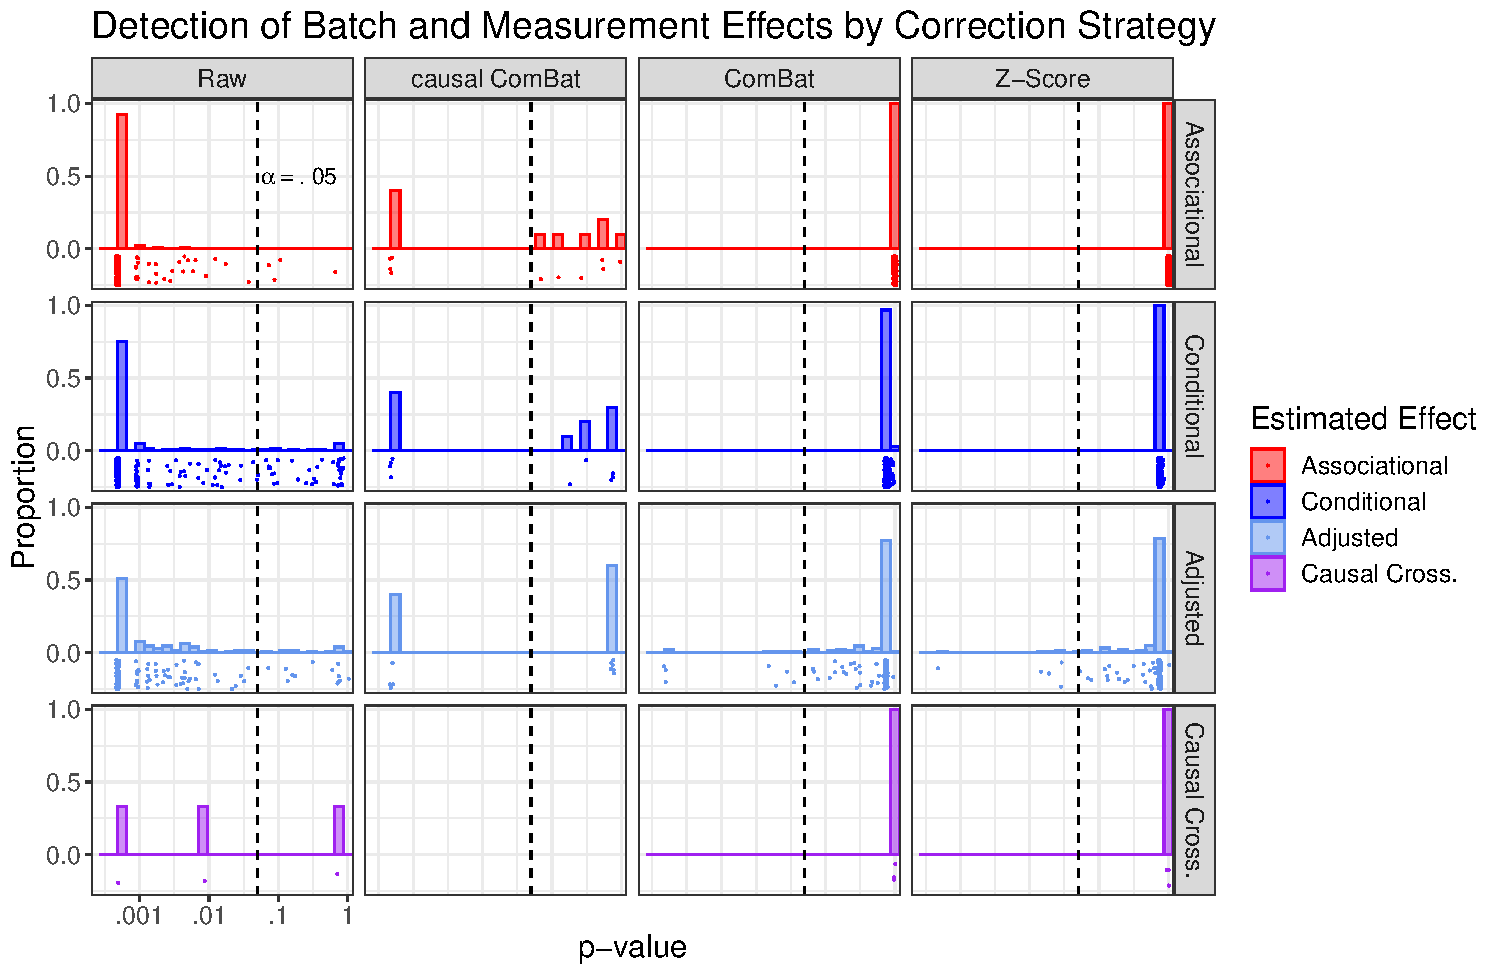
\includegraphics[width=\linewidth]{Figures/Supplement/hist_full.pdf}
    \caption{Empirical distribution of $p$-values for each estimated effect type by batch correction strategy.}
    \label{fig:site_hists_full}
\end{figure}

In Figure \ref{fig:site_hists_full}, we examine the prevalence of effects between different studies. It is important to note that whereas Causal \Combat\ can only be run on the American Clique, both \Combat\ and $Z$-scoring can be run on all studies. Recall that associational effects investigate whether \textit{any} batch effects are present between pairs of studies (either measurement- or demographics-related). Both \Combat\ and $Z$-scoring eliminating nearly \textit{all} variability between pairs of studies suggests that \Combat\ and $Z$-scoring are eliminating variability that is directly related to natural biological variability, which is not a favorable outcome. For both strategies, associational effects are not significant for 100\% of comparisons. This is because the studies differ on the basis of demographic covariates possessing signal, and therefore observing no associational batch effects after correction implies we have removed demographic signal. On the other hand, limiting oneself to only pairs of studies in which adjusted effects are estimable with Causal \Combat\ may offer a solution to this undesirable property of $Z$-scoring and naive \Combat.
\end{comment}


{\edits{\section{Simulations}
\label{app:sims}
\subsection{Batch Effect Detection Simulations}
\label{app:sim_effect}

{\edits{Simulations illustrating the sensitivity (high testing power when a causal effect is present) and specificity (tests which do not falsely detect effects) of \ccdcorr~for causal effect detection are in \citet{Bridgeford2023Jul}.}}


{\edits{\subsection{Batch Effect Removal Simulations}
\label{app:sim_batch_adj}

$n=400$ points are sampled from Batch $0$ or Batch $1$ with probability $0.5$; e.g. $T_i \distas{iid} \Bern{0.5}$. 

\subsubsection{Covariate distributions}
For each row, the covariate distributions are:

\paragraph*{I. Overlap} The covariate distribution is $X_i \distas{iid} 2\Beta{2, 2} - 1$.

\paragraph*{II. Moderate Overlap} The covariate distribution is:
\begin{align*}
    X_i | T_i = t \distas{d} \begin{cases}
        2\Beta{2, 6}-1 & t = 0 \\
        2\Beta{6, 2}-1 & t = 1
    \end{cases}
\end{align*}

\paragraph*{III. Limited Overlap} The covariate distribution is:
\begin{align*}
    X_i | T_i = t \distas{d} \begin{cases}
        2\Beta{2, 12}-1 & t = 0 \\
        2\Beta{12, 2}-1 & t = 1
    \end{cases}
\end{align*}

\subsubsection{Simulation contexts}
We investigate these in four simulation contexts, where for all simulations, $\epsilon_i \distas{iid} \Norm{0, 1}$:

\paragraph*{Non-linearity} A sigmoidal relationship between the covariate and the outcome. The outcome is:
\begin{align*}
    Y_i = 4\text{sigmoid}(8X_i) + T_i + \frac{1}{2}\epsilon_i,
\end{align*}

where $\text{sigmoid}(x)$ is the non-linear sigmoid function; e.g.:
\begin{align*}
    \text{sigmoid}(x) &= \frac{1}{1 + \exp(-x)}.
\end{align*}
The effectiveness of batch effect correction methods for the non-linearity setting are shown in Figure \ref{fig:sim_nlin_adjust}.

\paragraph*{Symmetric non-monotonicity} A gaussian non-monotonic relationship between the covariate and the outcome. The outcome is:
\begin{align*}
    Y_i = \varphi\parens*{X_i, \mu=0, \sigma=\frac{1}{2}} + T_i + \frac{1}{2}\epsilon_i,
\end{align*}

where $\varphi(x, \mu, \sigma)$ is the probability density function of the Normal distribution:
\begin{align*}
    \varphi(x, \mu, \sigma) &= \frac{1}{\sigma \sqrt{2\pi}}\exp\set*{\parens*{\frac{x - \mu}{\sigma}}^2}
\end{align*}
We call it ``symmetric'' because $\mu = 0$, which leads to the both the covariate/outcome relationship and the covariates themselves being symmetric about $x=0$. The effectiveness of batch effect correction methods for the symmetric non-monotonicity setting are shown in Figure \ref{fig:sim_nlin_adjust_nm_sym}.

\begin{figure}[h]
    \centering
    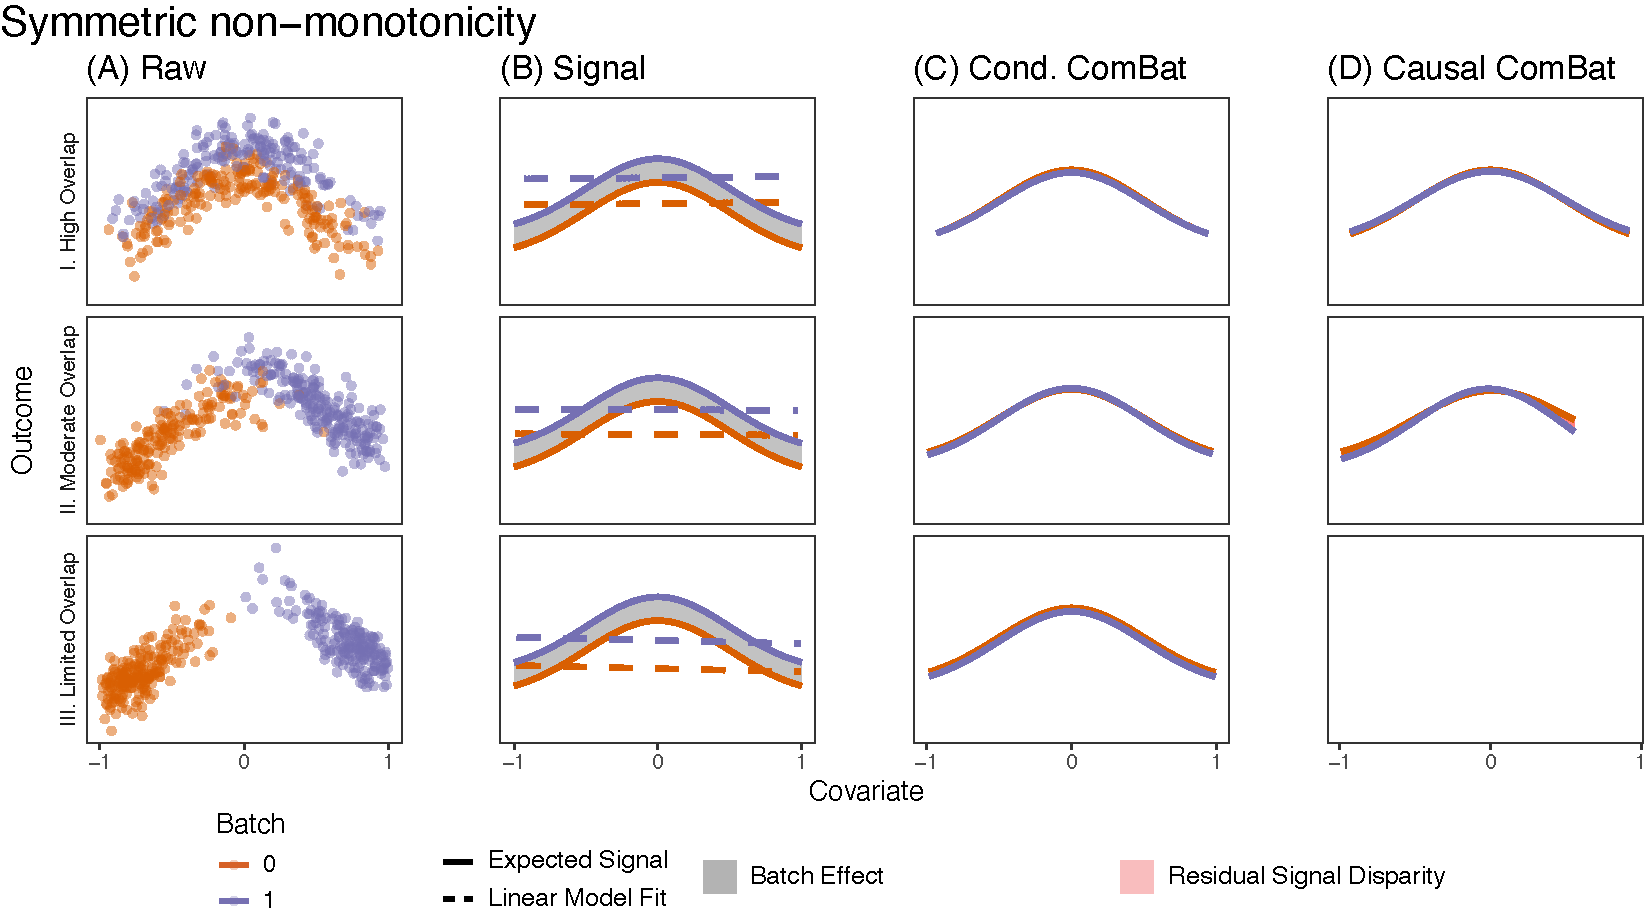
\includegraphics[width=\linewidth]{Figures/Supplement/Simulations/sim_nlin_adjust_nm_sym.pdf}
    \caption{A symmetric non-monotonicity about $x=0$. \ccombat~provides reasonable results when the non-monotonicity and the covariate distributions (for each batch) are symmetric about the same value (here, $x=0$). In high balance the MAAD of \ccombat~and \cccombat~are $0.076$ and $0.051$ (\cccombat~better $67.6\%$ of the time), in moderate balance are $0.179$ and $0.173$ (\cccombat~better $50.9\%$ of the time), and in limited overlap are $0.358$ and $0.289$ (\cccombat~better $66.7\%$ of the time) with \cccombat~only executing in $36$ simulations.}
    \label{fig:sim_nlin_adjust_nm_sym}
\end{figure}

\paragraph*{Asymmetric non-monotonicity} A gaussian non-monotonic relationship between the covariate and the outcome. The outcome is:
\begin{align*}
    Y_i = \varphi\parens*{X_i, \mu=-0.5, \sigma=\frac{1}{2}} + T_i + \frac{1}{2}\epsilon_i.
\end{align*}
We call it ``asymmetric'' because $\mu = -0.5$, which leads to the effect not being symmetric about $x = 0$ (whereas the covariates are, by construction, symmetric about $x=0$). The effectiveness of batch effect correction methods for the asymmetric non-monotonicity setting are shown in Figure \ref{fig:sim_nlin_adjust_nm_asy}.

\begin{figure}[h]
    \centering
    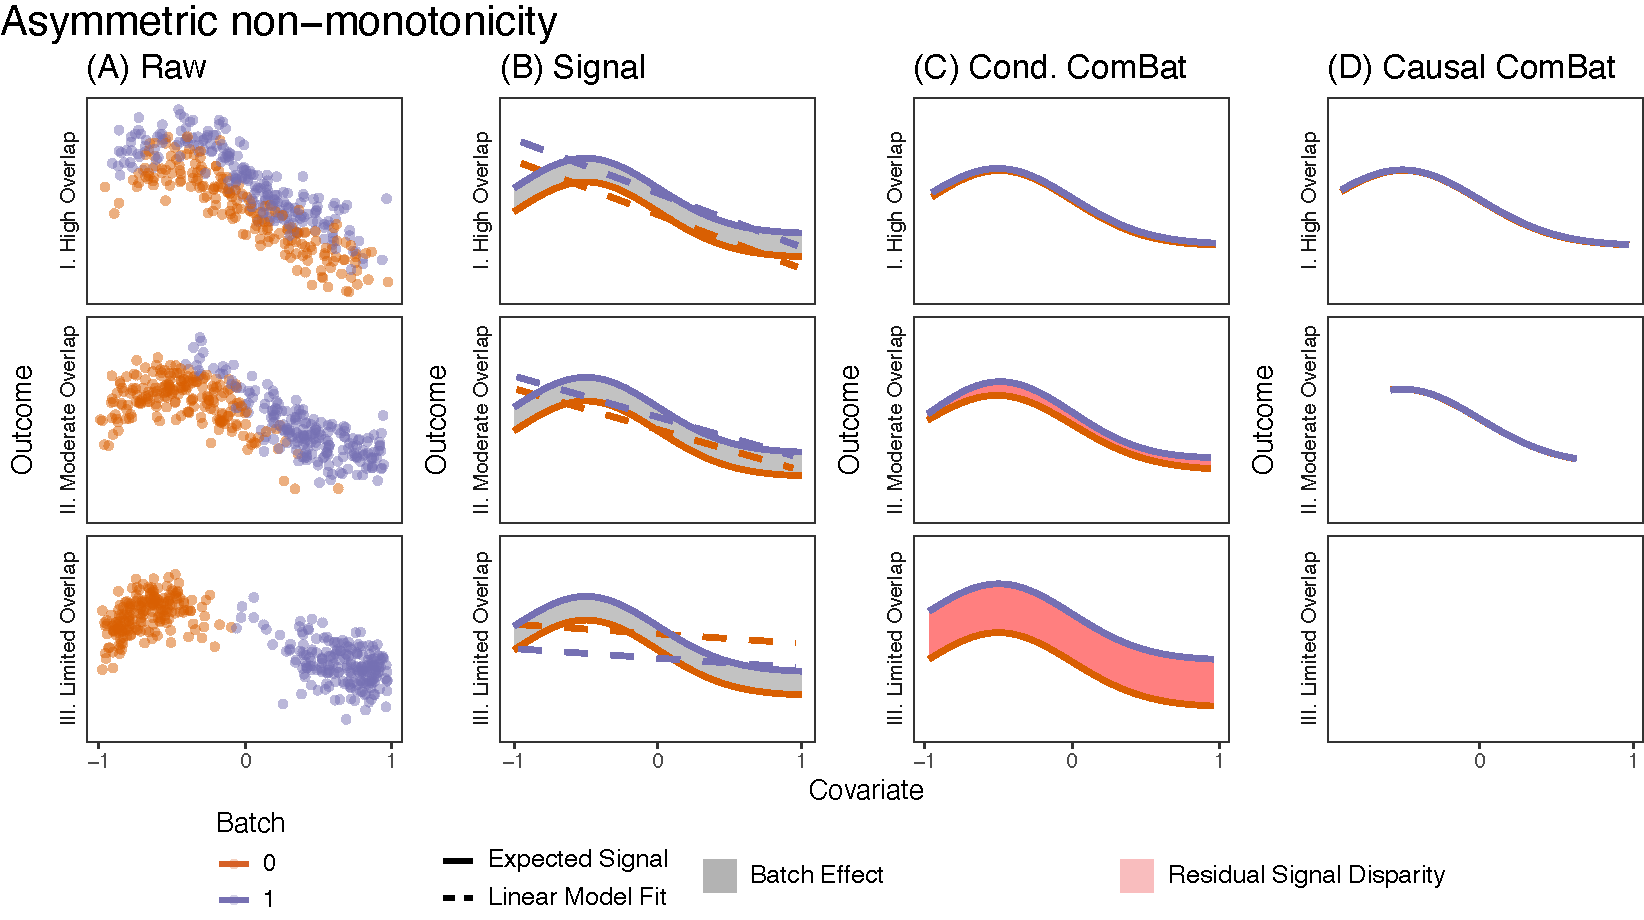
\includegraphics[width=\linewidth]{Figures/Supplement/Simulations/sim_nlin_adjust_nm_asy.pdf}
    \caption{An asymmetric non-monotonicity in which the non-monotonicity is not symmetric about $x=0$, while the covariate distributions (for each batch) are symmetric about $x=0$. \ccombat~ struggles and worsens the batch effect as the covariate balance decreases, while \cccombat~is able to work as long as there are moderate amounts of covariate overlap. In high balance the MAAD of \ccombat~and \cccombat~are $0.0497$ and $0.0421$ (\cccombat~better $59.5\%$ of the time), in moderate balance are $0.074$ and $0.130$ (\cccombat~better $99.7\%$ of the time), and in limited overlap are $2.61$ and $0.407$ (\cccombat~always better) with \cccombat~only executing in $33$ simulations.}
    \label{fig:sim_nlin_adjust_nm_asy}
\end{figure}


\paragraph*{Symmetric non-monotonicity, asymmetric covariates} A gaussian non-monotonic relationship between the covariate and the outcome, and a different covariate distribution from the rest of the simulations. The covariate distribution is:
\begin{align*}
    X_i | T_i = t \distas{d} \begin{cases}
        2\Beta(2, 2) - 1 & t = 0 \\
        2Beta(b, 2) - 1 & t = 1
    \end{cases}
\end{align*}
where $b = 2$, $b=6$, and $b=12$ for the overlap, moderate, and limited conditions, respectively.

The outcome is:
\begin{align*}
    Y_i = \varphi\parens*{X_i, \mu=0, \sigma=\frac{1}{2}} + T_i + \frac{1}{2}\epsilon_i.
\end{align*}
This time, the non-monotonicity is symmetric, but the covariate distributions are increasingly asymmetric. The effectiveness of batch effect correction methods for the asymmetric non-monotonicity setting are shown in Figure \ref{fig:sim_nlin_adjust_nm_sym_asy}.

\begin{figure}[h]
    \centering
    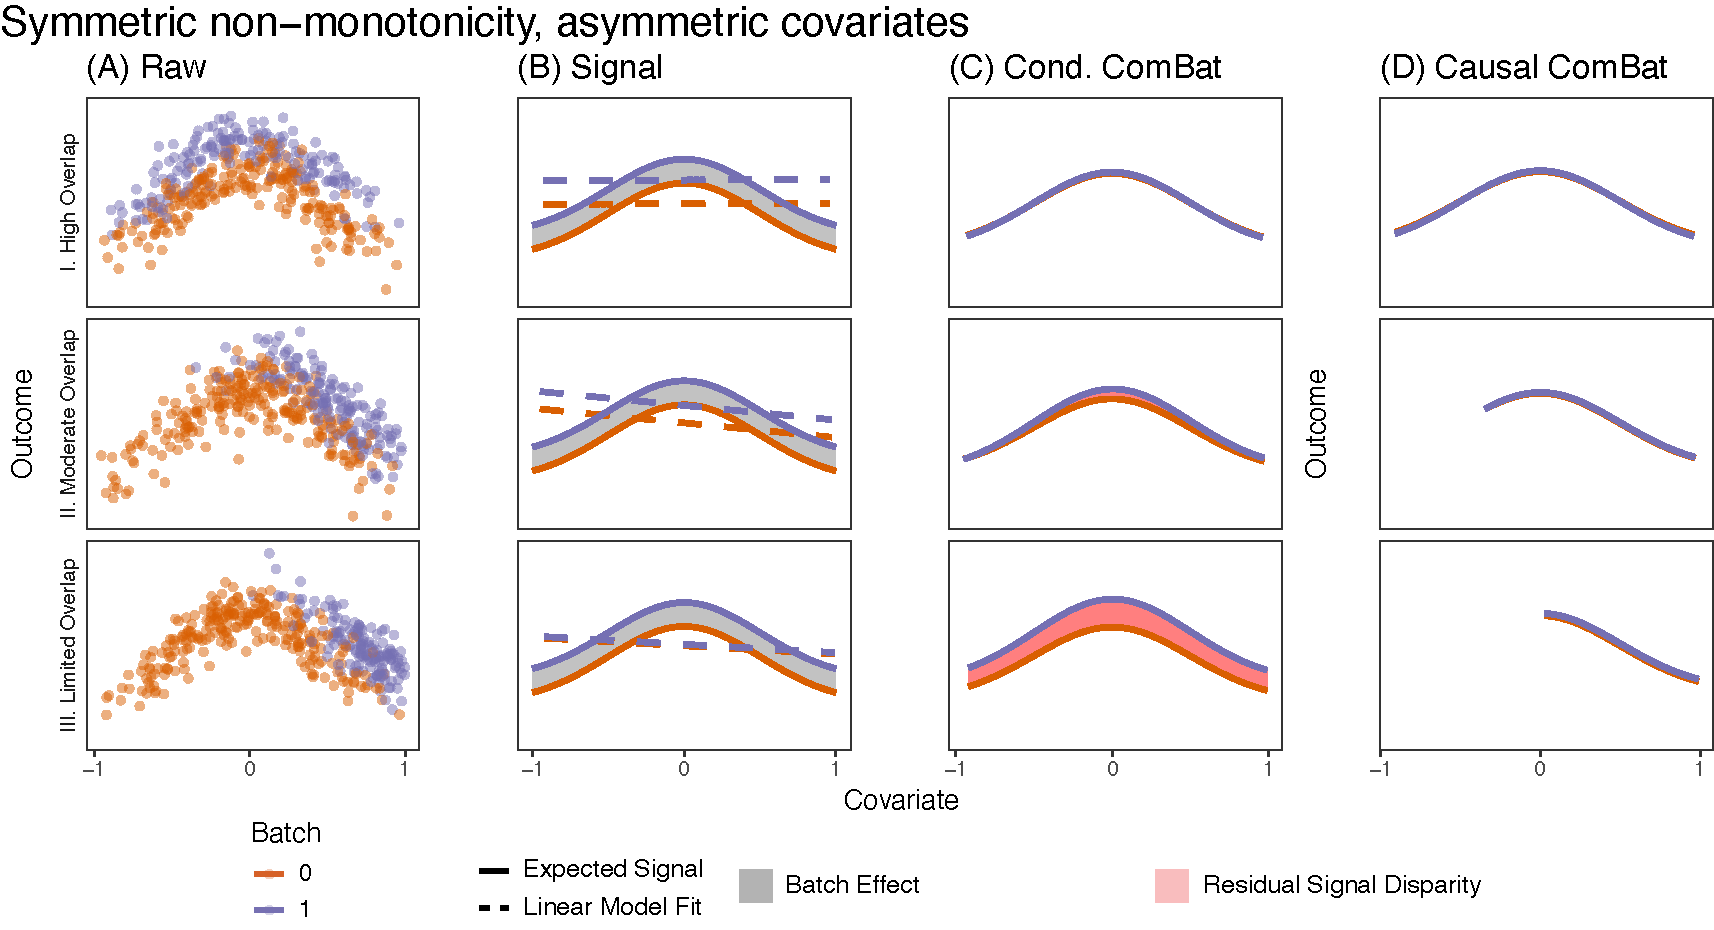
\includegraphics[width=\linewidth]{Figures/Supplement/Simulations/sim_nlin_adjust_nm_sym_asy.pdf}
    \caption{A symmetric non-monotonicity about $x=0$, but the covariate distribution is no longer symmetric about $x=0$. \ccombat~struggles to remove the batch effect and leaves a residual signal disparity, but \cccombat~is able to address the batch effect within a range of covariate overlap. In high balance the MAAD of \ccombat~and \cccombat~are $0.075$ and $0.0506$ (\cccombat~better $65.8\%$ of the time), in moderate balance are $0.181$ and $0.0751$ (\cccombat~better $96.0\%$ of the time), and in limited overlap are $0.84$ and $0.106$ (\cccombat~always better). Due to the fact that the covariate distribution for batches $0$ and $1$ overlap for this simulation, \cccombat~always executes.}
    \label{fig:sim_nlin_adjust_nm_sym_asy}
\end{figure}


\paragraph*{Linear} A linear relationship between the covariate and the outcome. The outcome is:
\begin{align*}
    Y_i = -2\parens*{X_i - 1} + T_i + \frac{1}{2}\epsilon_i.
\end{align*} The effectiveness of batch effect correction methods for the linear setting are shown in Figure \ref{fig:sim_lin_adjust}.

\begin{figure}[h]
    \centering
    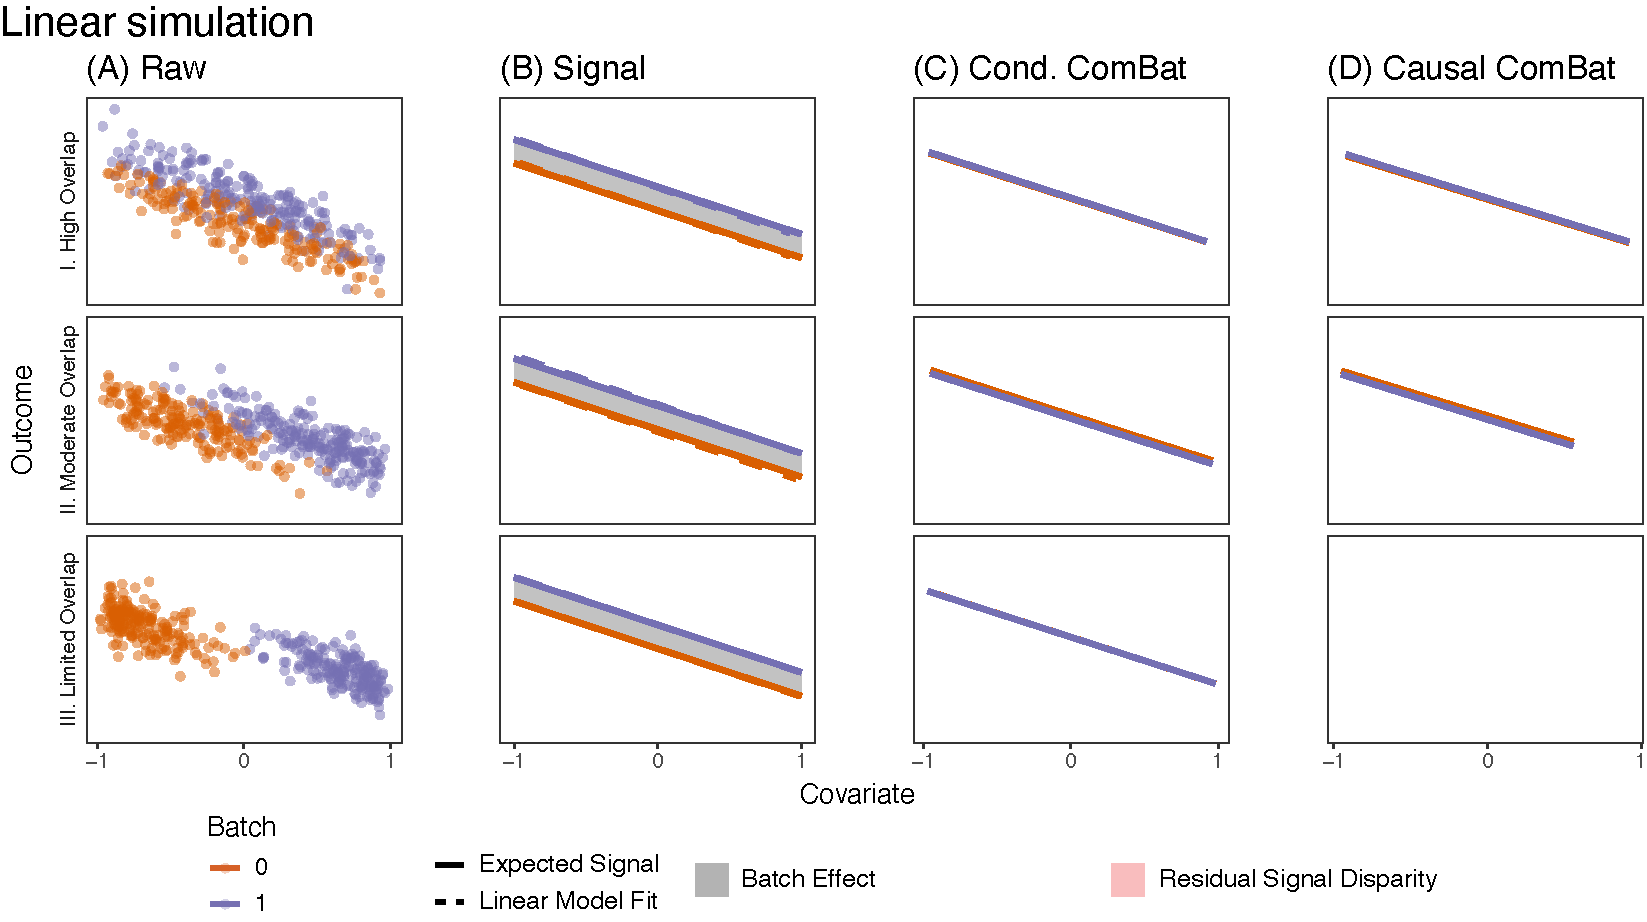
\includegraphics[width=\linewidth]{Figures/Supplement/Simulations/sim_lin_adjust.pdf}
    \caption{A linear simulation in which the assumptions of \ccombat~are perfectly satisfied. In high balance the MAAD of \ccombat~and \cccombat~are $0.035$ and $0.0375$ (\cccombat~better $42.5\%$ of the time), in moderate balance are $0.074$ and $0.113$ (\cccombat~better $33.1\%$ of the time), and in limited overlap are $0.145$ and $0.292$ (\cccombat~better $23.1\%$ of the time) with \cccombat~only executing in $39$ simulations.}
    \label{fig:sim_lin_adjust}
\end{figure}

\subsection{Mean Average Absolute Difference (Mean AAD)}
\label{app:maad}
To evaluate the effectiveness of each batch effect correction technique on simulated data, we compute the true data expected signal for each covariate level; e.g., $\expect{Y_i(t) | x}$ for each batch $t$ and each covariate level $x$. Since $\epsilon_i$ has mean $0$, this would be the quantity:
\begin{align*}
    \expect{Y_i(t) | x} &= f(x) + t,
\end{align*}
where $f$ is the covariate/outcome relationship (possibly incorrectly modeled). Since $x$ is continuous, we compute this value for $x$ across $B=200$ evenly spaced breakpoints for evaluation. Given a set of samples, we train a batch effect correction model, and fit the trained model to the expected signal for each covariate level, leaving us with adjusted expected signal for each batch, which we denote by $V_i(t, x)$. In theory, if the batch effect correction technique removes the batch effect as modeled, $V_i(1, x) \approx V_i(0, x)$ for all $x$. To evaluate each technique, we consider the average absolute difference for each trial $r$ of $1000$ trials:
\begin{align*}
    d_r &= \frac{1}{B} \sum_{x \in \mathcal X}\left|v_i(1, x) - v_i(0, x)\right|,
\end{align*}
and the magnitudes of $d_r$ are annotated in the plots (shaded red boxes) for a single simulation. We compute the mean AAD as:
\begin{align*}
    d &= \frac{1}{r}\sum_{r \in [R]} d_r.
\end{align*}
A value of $0$ corresponds to the batch effect being completely eliminated (the expected signal for each batch after correction is identical), a value of $1$ would equate to the residual disparity between the expected signals being the same as before batch effect correction, and a value $> 1$ corresponds to the residual disparity between the expected signals \textit{exceeding} the original batch effect.

\subsection{Causal \Combat~outperforms Conditional \Combat~on simulated data}

Across all simulations, simulated measurements are collected from an additive gaussian model with either a linear (Figure \ref{fig:sim_lin_adjust}), non-linear (Figure \ref{fig:sim_nlin_adjust}), or non-monotonic (Figure \ref{fig:sim_nlin_adjust_nm_sym}, Figure \ref{fig:sim_nlin_adjust_nm_asy}, and Figure \ref{fig:sim_nlin_adjust_nm_sym_asy}) covariate/outcome relationship, with a batch-specific offset. We performed these simulations for cases where the covariate distributions overlap (row I), moderately overlap (row II), and have limited overlap (row III). When the assumptions between the covariate and the measurements are correct, covariate overlap is irrelevant, as the covariate-specific signal can be extrapolated successfully across the entire range of the covariate. When the assumptions between the covariate and the measurements are incorrect, the batch effect can still be removed, as shown in column (D), when further conditions are satisfied, such as:
\begin{enumerate}[leftmargin=*]
    \item covariate distributions are matched: can be conceptualized as the inaccurate assumptions of the model, in effect, being uniformly \textit{misrepresented} by the model in each of the two batches, which \textit{still} enables a consistent estimate of the batch effect to be estimated and removed. \cccombat~attempts to enforce this approach through matching. We explored the implications of this in Figure \ref{fig:sim_nlin_adjust} and Figure \ref{fig:sim_nlin_adjust_nm_asy}.
    \item the covariate distributions (and the covariate/outcome relationship) are symmetric about the same point: again, the idea here is that intuitively, the the inaccurate assumptions of the model must be uniformly misrepresented by the model in the two batches. This is a pre-hoc condition and relates directly to the specific underlying true veridical signal, and is difficult to exploit practically. We explore the implications of this in Figure \ref{fig:sim_nlin_adjust_nm_sym} and Figure \ref{fig:sim_nlin_adjust_nm_sym_asy}.
\end{enumerate}

As shown in the simulations in Figure \ref{fig:sim_nlin_adjust} and Figure \ref{fig:sim_nlin_adjust_nm_asy}, these artifacts can be arbitrarily large depending on the nature of the incorrect assumption. In these examples, the residual signal disparity introduced by \ccombat~in limited overlap cases (row III) dwarfs the magnitude of the original batch effect, and is of similar magnitude with moderate covariate overlap (row II). 

On the other hand, \cccombat~first pre-aligns the covariate distributions, and even with model misspecifications, is able to successfully remove a batch effect for the subset of the covariate space with sufficient covariate overlap. Importantly, causal strategies \textit{explicitly prohibit} learning about data which falls outside of the region of demographic overlap. When overlap conditions are not met for a portion of the sample space, causal strategies do not do anything, as is typically the case for most of the illustrated similations in the ``Limited Overlap'' condition. In this sense, causal techniques are therefore more conservative for batch effect detection and mitigation. We believe this to be favorable for batch effect detection and mitigation as, in practice, it is effectively impossible to tell whether the implicit or explicit assumptions of the model for batch effect correction~are sufficient or not, and almost impossible for our model to account for all ways a batch effect could manifest in high-dimensional data (such as higher order correlations, non-linearities, variance differences) given a finite sample. This presents an enormous point of caution when applying batch effect removal techniques to high-dimensional datasets with confounding, as it is infeasible to explore whether extrapolatory modeling assumptions are within reason on a dimension-by-dimension (or, higher-order) basis.}

}

\paragraph{Addressing the batch effect}
One way to characterize the batch effect in univariate contexts (and within our simulations) would be analogous to the average treatment effect \cite{Rosenbaum1983Apr}; e.g.:
\begin{align*}
    \text{ATE} = \expect{Y(1) - Y(0)}
\end{align*}
For all simulations, by construction the ATE is $1$ and does not depend on the covariates.

By definition, a difference in the expectations implies that $Y(1) \overset{\mathcal D}{\neq} Y(0)$, and a batch effect is present by Definition \ref{def:causal_batch_informal}.

It is well understood in the statistical literature that for models of the form $Y_i = g(X_i) + \beta T_i + Z_i$ where $Z_i \distas{iid} \Norm{\mu, \Sigma}$, that as long as either the strong ignorability condition \cite{Rosenbaum1983Apr} or $f$ is known, the adjustment factor $\hat\beta_1 - \hat \beta_0$ will be a consistent and unbiased estimate of the ATE \cite{Rosenbaum1983Apr, vdv}. For a non-technical explanation in words, we can obtain reasonable estimates of the ATE in one of three ways (and consequently, account for the batch effect):
\begin{enumerate}[leftmargin=*]
    \item Extrapolation: if we know $g(x)$, then we can ``guess'' what $\expect{Y_i(t)|x}$ looks like for values of $x$ that do not exist in our batch, by appropriate estimation of $g$ via the elements of our dataset that we \textit{do} have. In this case, where the model is linear, extrapolation can be performed by linear regression. Once we have identified $g(x)$, we can extrapolate what $g(x)$ looks like for values of $x$ which fall outside the range of our dataset, as in Figure \ref{fig:sim_lin_adjust}; particularly, noting cells (C).II and (C).III.
    \item Use asymptotics: if we do not know $g(x)$ but we can reasonably assume that the strong ignorability condition holds, we can leverage asymptotic statistics to conclude that we can still adequately estimate the CATE. Proofs of this result can be found in \cite{Rosenbaum1983Apr,Rosenbaum1985}. In this particular case, $X_i \indep T_i$, which implies the strong ignorability condition \cite{Rosenbaum1983Apr}. For more trivial reading specific to the case where $X_i \indep T_i$, see \cite{vdv}. This result is exhibited in the simulations for Figure \ref{fig:sim_nlin_adjust} and Appendix Figure \ref{fig:sim_nlin_adjust_nm_asy} looking at column (D) compared to column (C), and noting that causal pre-processing procedures tend to produce a reasonable result (while non-causal conditional procedures with a model misspecification do not).
    \item The covariate distribution is symmetric about the same point that a non-monotonicity is symmetric: in this extremely special case, we have that $f(x | 1) = f(-x | 0)$, and $f(y(0) | x) = f(y(1) | -x)$ for every $x$. This result is exhibited by way of comparison of Figures \ref{fig:sim_nlin_adjust_nm_sym} and Figure \ref{fig:sim_nlin_adjust_nm_asy}, and noting that while Figure \ref{fig:sim_nlin_adjust_nm_sym}(C).III is able to arrive at a reasonable solution, Figure \ref{fig:sim_nlin_adjust_nm_asy}(C).III does not.
\end{enumerate}
By a similar argument, the estimated batch disparity can also be consistently estimated in either of these contexts. In these cases, removal of the estimated offset associated with the particular batch of a measurement is a reasonable approach to removal of the estimated batch effect.

Simulations in which the assumption about $f(x)$ is incorrect and $X_i$ is distributed conditionally on $T_i$ (and consequently, the strong ignorability condition will not hold), will not necessarily yield a reasonable estimate of the ATE.
}

\section{Overlap of Empirical Covariates}
\label{app:overlap}

The empirical overlap of the covariate distributions is difficult to compute in the case of data without making heavy parametric assumptions. For this reason, we turn to the distribution-free overlapping index \cite{Pastore2019}. The distribution free overlapping index, $\hat v_{kl}$, is computed by first approximating the density of the distribution of the measured covariates for each dataset $D$, $X = (A, S, C)$, where $A$ is a random variable whose realizations $a \in \mathcal A$ are ages, $S$ is a random variable whose realizations $s \in \mathcal S$ are sexes (M or F), and $C$ is a random variable whose realizations $c \in \mathcal C$ denote continent, using the base \texttt{R} function \texttt{stats::density}. The random variable $D$ has realizations $d \in \mathcal D$ whose realizations denote dataset. The density $f\parens*{a| S = s, C = c, D = d}$ is the conditional density of age, conditional on the individual's sex being $s$, continent of measurement being $c$, and dataset being $d$. The mass $\prob{S = s | C = c, D = d}$ is the conditional mass of sex, conditional on the individual's continent of measurement being $c$, and dataset being $d$. Finally, the mass $\prob{C = c | D = d}$ represents the conditional mass of an individual's continent of measurement being $c$, conditional on the dataset being $d$ ($0$ or $1$ for all $d$, since all individuals from dataset $d$ are either measured on continent $c$ or not). An estimate of the overlap between the two densities, $\hat v_{kl}$ between datasets $k$ and $l$, is computed using the formula:
\begin{align*}
    \hat v_{kl} &= \sum_{c \in \mathcal C}\min\parens*{\hat {\mathbb P}\parens*{C = c | D = k}, \hat{\mathbb P}\parens*{C = c | D = l}}\sum_{s \in \set*{\text M, \text F}}\min\parens*{\hat{\mathbb P}\parens*{S = s | C = c, D = k},\hat {\mathbb P}\parens*{S = s | C = c, D = l}}\bigg[ \\
    &\undereq\integral{\mathcal A}{}{\min\parens*{\hat f\parens*{a | S = s, C = c, D = k}, \hat f\parens*{a | S = s, C = c, D = l}}}{a}\bigg]
\end{align*}
which is obtained via numerical quadrature.

Intuitively, this can be conceptualized as representing the mass of the "area under the curve" which is shared by the two densities for datasets $k$ and $l$.

\begin{figure}[h!]
    \centering
    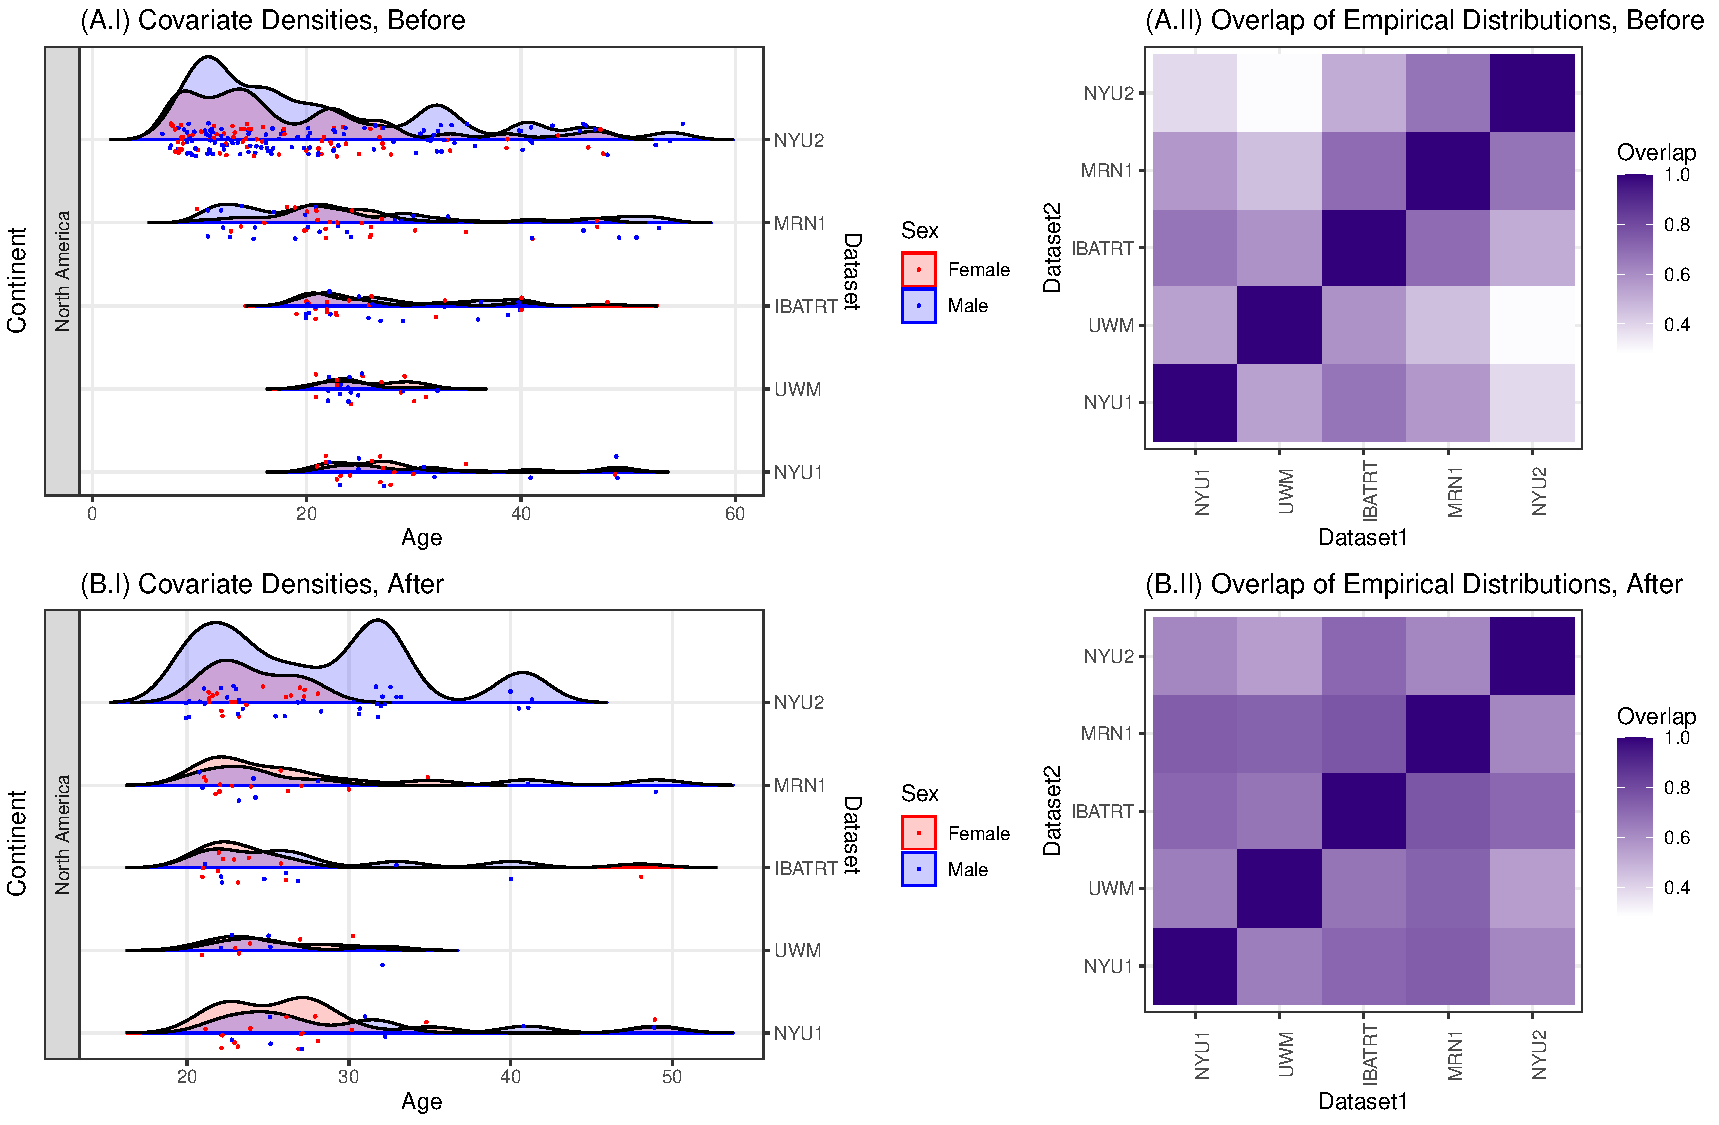
\includegraphics[width=\linewidth]{Figures/Supplement/ov_app.pdf}
    \caption{\textbf{The overlap of the empirical covariate distributions for the American Clique, before and after adjustment}. \textbf{(A)} The empirical distributions of the covariates before adjustment. \textbf{(B)} The empirical overlap of the covariate distributions after the adjustment procedure is applied, as discussed in Appendix \ref{app:cross_effect}.}
    \label{fig:overlap}
\end{figure}

\begin{figure}[h!]
    \centering
    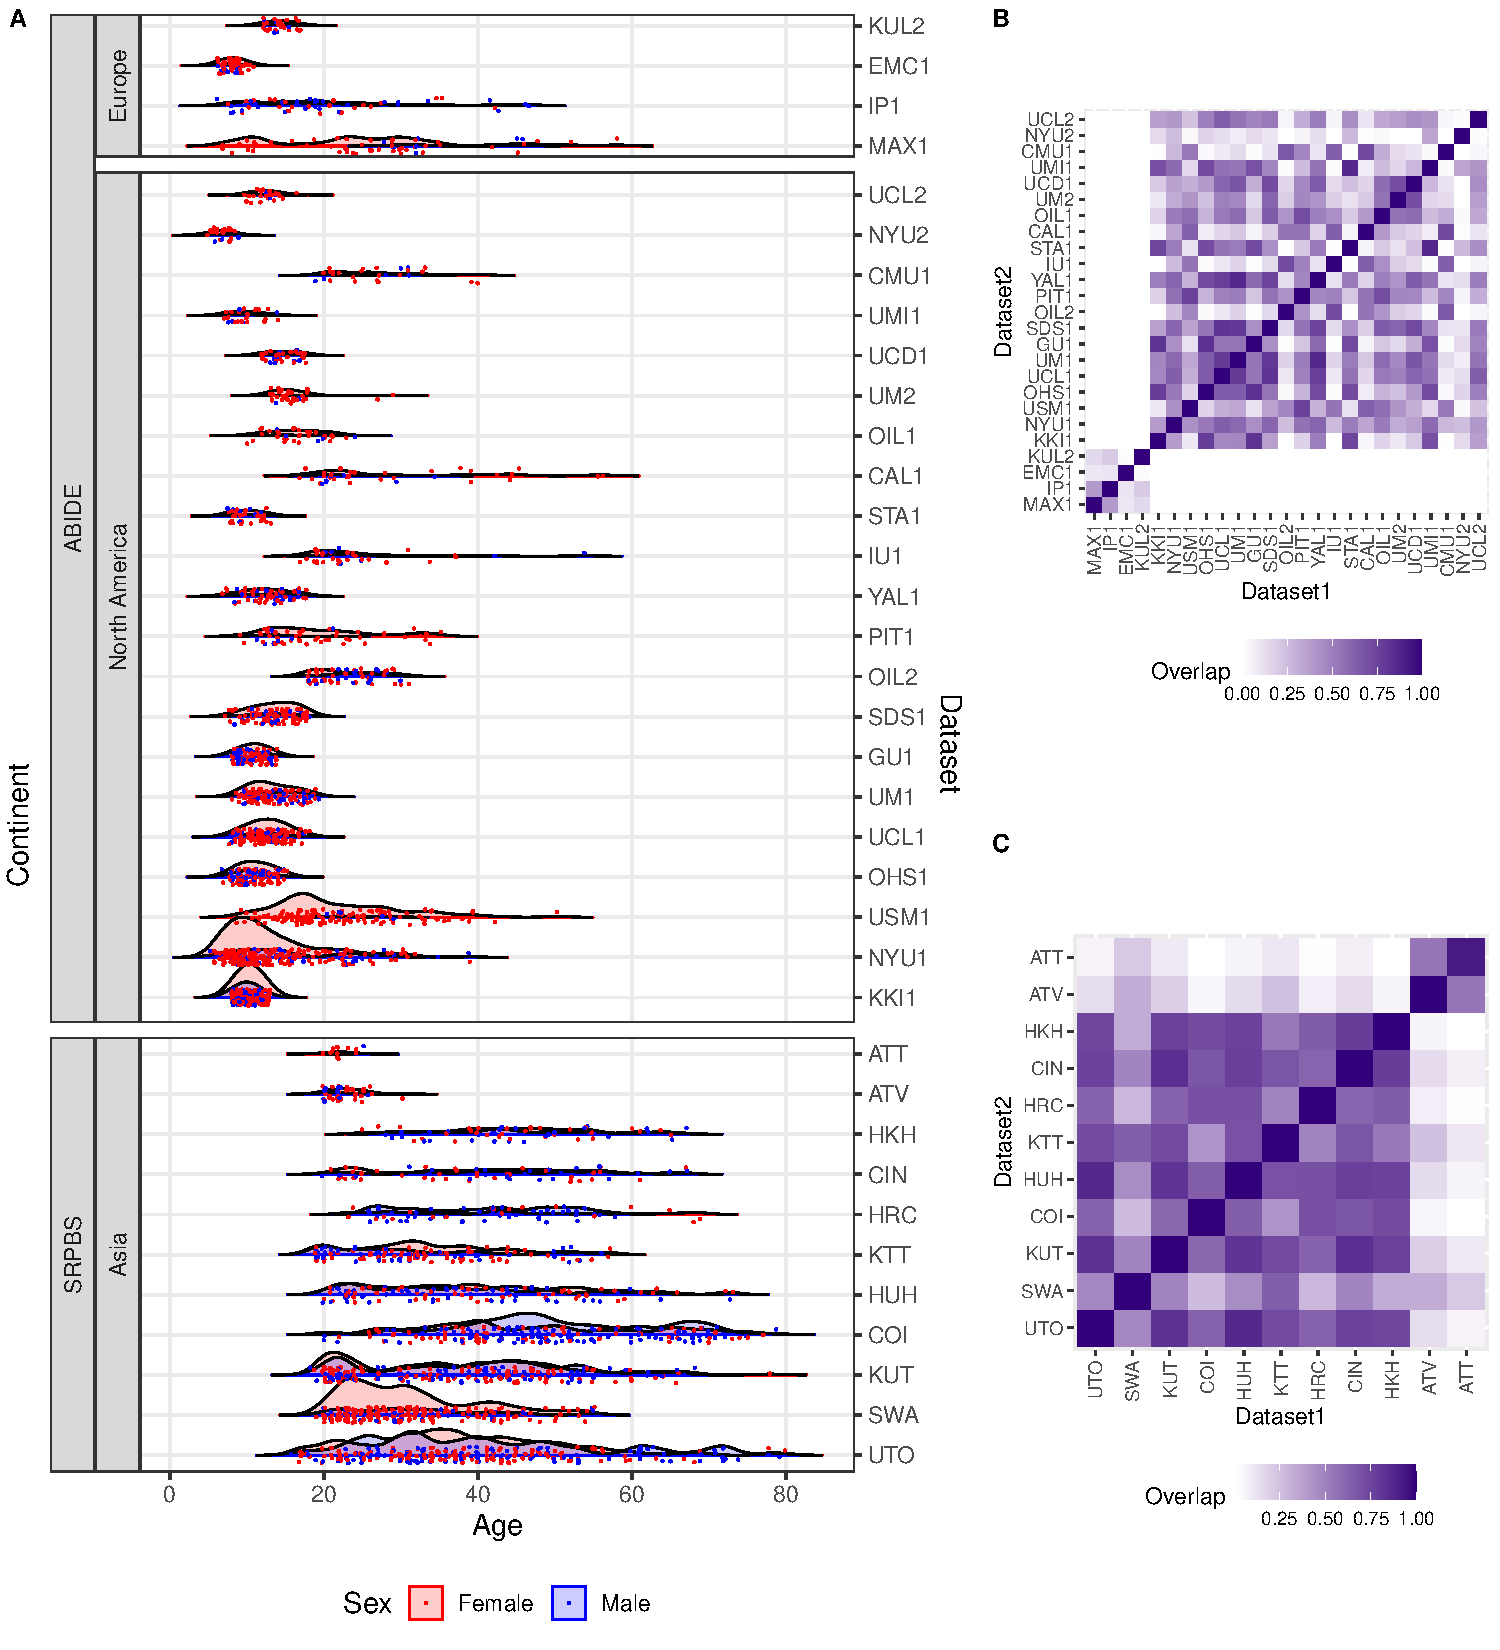
\includegraphics[width=\linewidth]{Figures/Supplement/mega_overlap.pdf}
    \caption{\textcolor{black}{\textbf{The overlap of the empirical covariate distributions for two mega-studies.} \textbf{(A)} The empirical distribution of covariates. \textbf{(B)} The overlap of covariate distributions given by the distribution-free overlapping index for ABIDE mega-study \cite{di2014autism, di2017enhancing}. \textbf{(C)} The overlap of covariate distributions given by the distribution-free overlapping index for the SRPBS mega-study. \cite{Yamashita2019Apr}. Like for the CoRR mega-study, while several pairs of sites have overlapping demographic distributions, many of the sites have extremely poor overlap in both mega-studies. In these cases, attempts to normalize for batch effects using model-based approaches like Conditional \Combat~would be subject to the pitfalls of Figure \ref{fig:sim_nlin_adjust}, Appendix \ref{fig:sim_nlin_adjust_nm_asy}, or Appendix Figure \ref{fig:sim_nlin_adjust_nm_sym_asy} if modeling assumptions are not reasonable.}}
    \label{fig:overlap2}
\end{figure}

\subsubsection{Batch Effects are reduced with Causal \Combat}

Here we investigate batch effects before and after correction. Figure  \ref{fig:site_hists} shows average connectomes from the MRN1 and IBATRT studies. With no correction, while the average connectomes appear similar between the two studies, a difference between the average connectomes is present (bottom row). Three different batch effect mitigation strategies ($Z$-scoring across features within a single batch, \Combat, and Causal \Combat) all appear to eliminate the differences between the average connectomes. $Z$-scoring has disrupted fundamental topological properties of the human connectome, as explored in detail in Appendix \ref{app:topological}. For this reason, we do not consider $Z$-scoring going forward, and focus instead on variations of the \Combat~procedure.

\begin{figure}[h!]
    \centering
    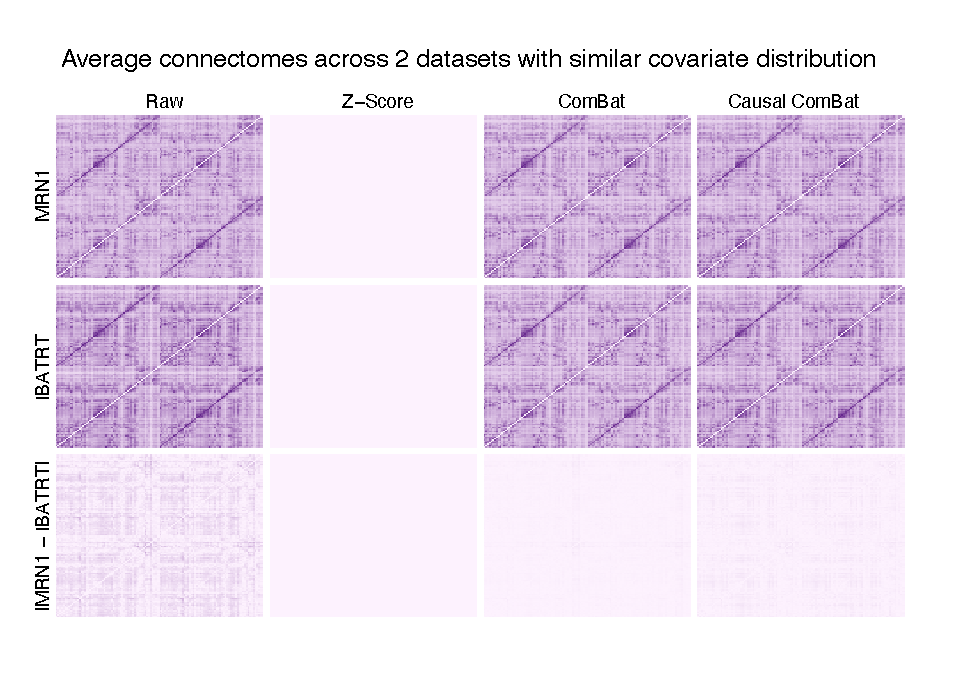
\includegraphics[width=.9\linewidth]{Figures/Content/site_effect_jk_2b.pdf}
    \caption{\textbf{Distribution of Detected Effects Before and After Correction}. A comparison of the average connectomes from two studies from the same continent, with similar sex and age distributions conditional on sex. While the \textit{Raw} average connectomes appear similar, the absolute difference between the two is appreciable. All of the three adjustment strategies reduce the absolute difference between the average connectomes for the two batches.}
    %\textbf{(B)} The difference between the average male and female connectome in the NYU2 study, compared to the difference between the average male connectome from the NYU2 study and the Utah1 study (all female). \Combat~has eliminated the sex disparity in favor of making average connectomes similar across studies.  \textbf{(C)} The difference between the average connectomes in the NYU2 study and the IBATRT study, across the raw, \Combat, and Causal \Combat~connectomes. Causal \Combat~has increased the disparity between the NYU2 study and the IBATRT study.}
    \label{fig:site_hists}
\end{figure}

\section{\Combat\ Preserves Topological Properties of fMRI Connectomes}
\label{app:topological}
% say Z-Score stuff first
The presence of two prominent topological \textit{signal effects} in human connectomes, homophily  and homotopy, are investigated in Figure \ref{fig:site_individual}. 
% avoid stuff like this
The left column of Figure \ref{fig:site_individual}A looks at the edges comprising these two disparate community structures. When edges are sorted by hemisphere, the homophilic effect is characterized by a modular two-block structure, with higher connectivity in the lower left and upper right blocks (dark red) than in the two off-diagonal blocks (pink). The homotopic effect is characterized by edges in the off-diagonal band (dark blue) showing higher connectivity than other edges within the connectome (light blue). The right column of Figure \ref{fig:site_individual}A looks at a single individual's connectome from the NYU2 study before and after correction. The homotopic property appears to be  preserved in only the \Combat\ connectomes, whereas $Z$-scored connectomes do not appear to preserve this property. In Figure \ref{fig:site_individual}B, these two properties are examined statistically for the individuals from the American Clique (Mann-Whitney $U$ Statistic, see Methods \ref{app:control} for details). Points falling along the diagonal line $y=x$ tend to have a similar signal effect before and after batch correction. Whereas \Combat~ strategies tend to preserve the homophilic and homotopic effects, $Z$-scoring tends to decrease these two topological properties of functional connectomes. This is noted by the fact that the majority of the points for $Z$-scoring across both effects tend to fall below the $y=x$ line, indicating that the effect size after $Z$-scoring is lower than the effect size in the raw connectomes.


\begin{figure}[h!]
    \centering
    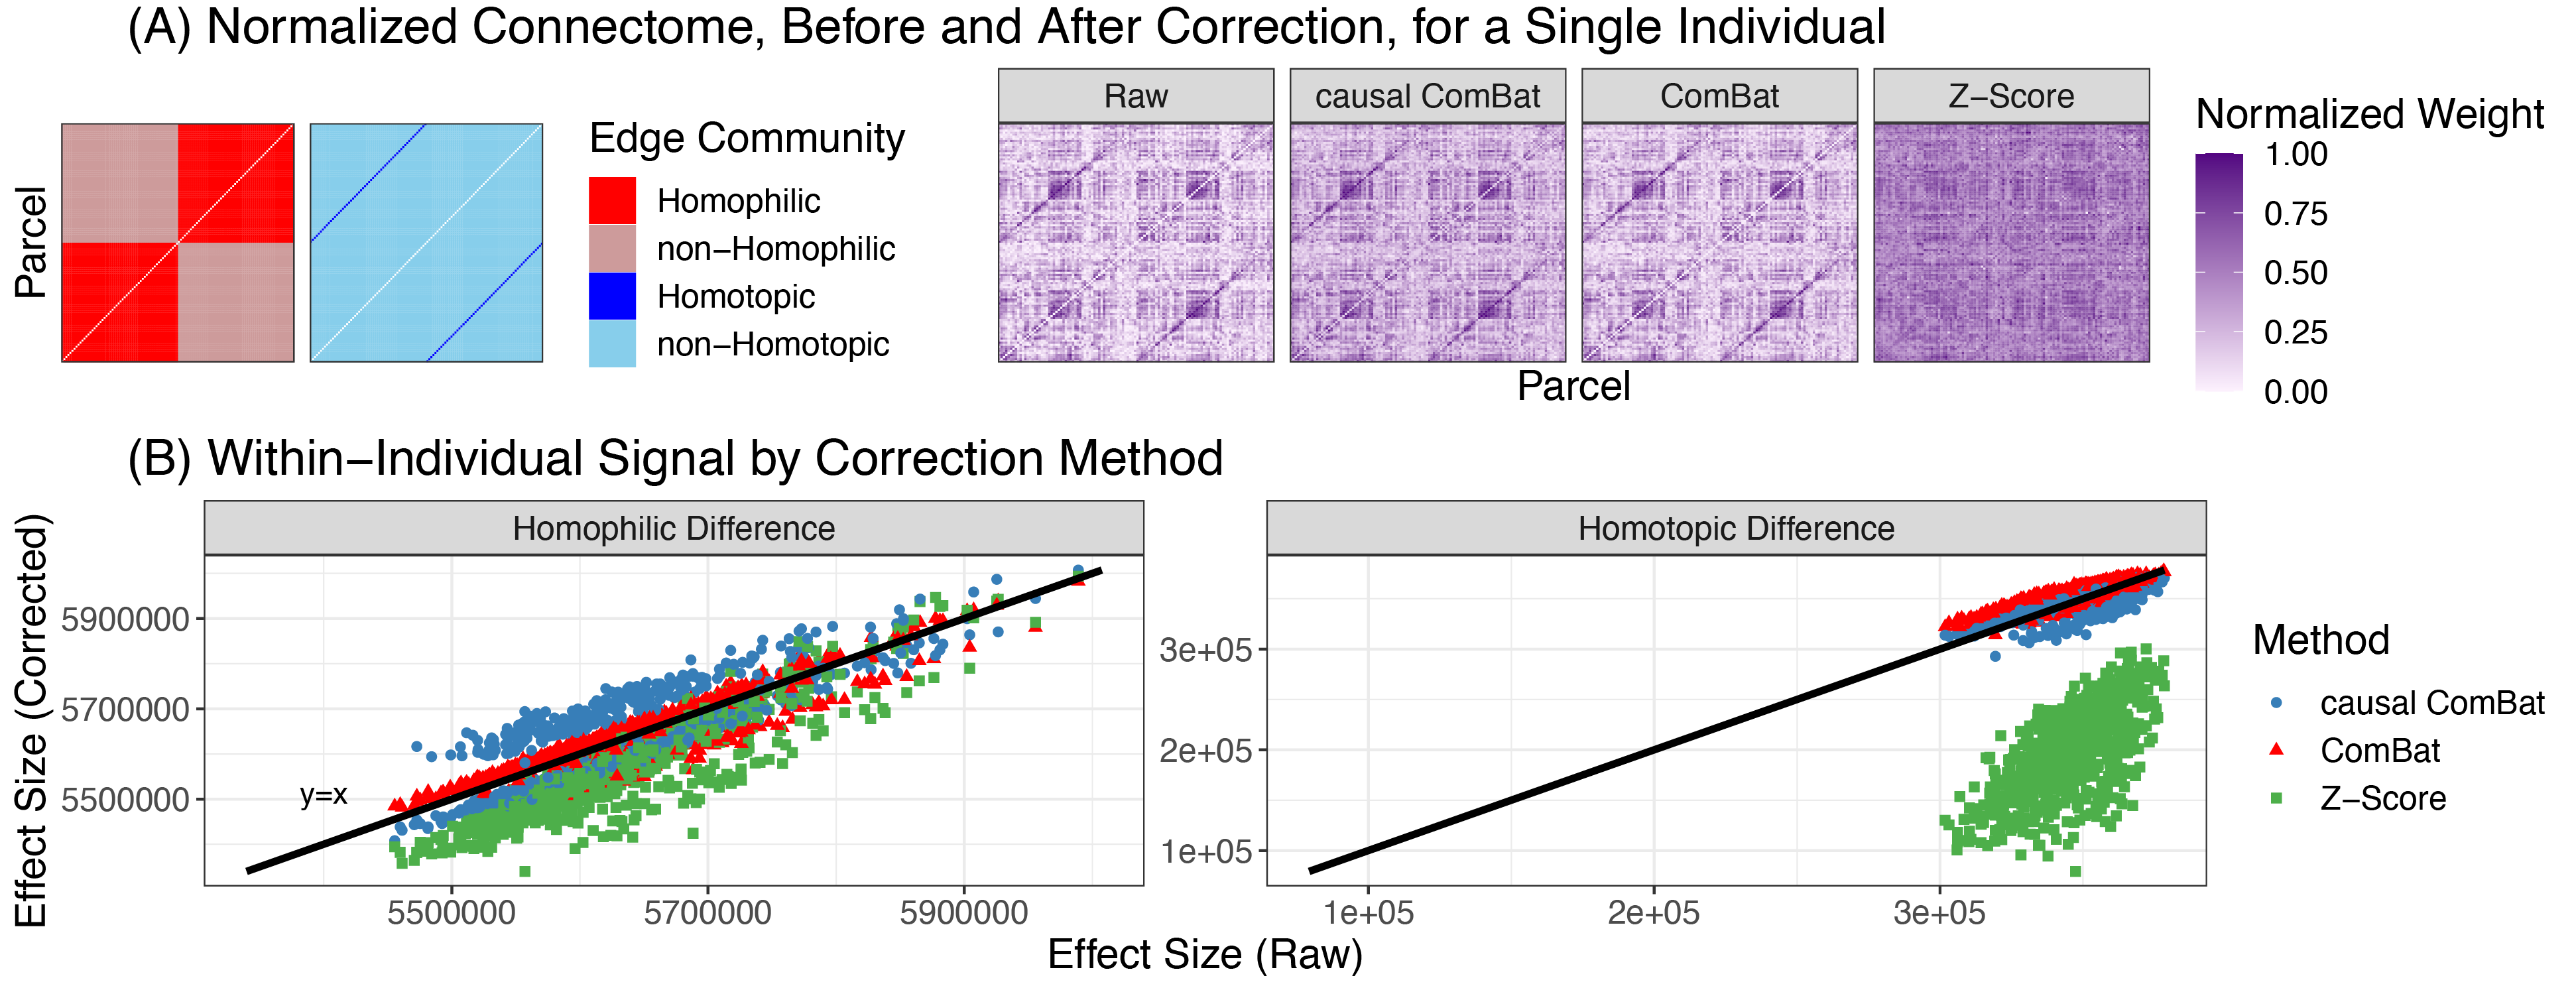
\includegraphics[width=\linewidth]{Figures/Supplement/Signal.png}
    \caption{\textbf{Preservation of Topological Properties of Connectomes after Batch Correction}. The presence of topological effects is explored in the context of the homophilic and homotopic differences in connectivity in the American Clique. \textbf{(A)} (\textit{Left}) A map indicating which edges are associated with homophilic/non-homophilic or homotopic/non-homotopic edge communities. %We look at connectomes only from those in which an adjusted site effect could be removed, from the American Clique \ref{sec:corr_descr}. 
    (\textit{Right}) The edge-weight normalized connectome associated with a single individual from the NYU2 study using each removal strategy. % The adjusted \texttt{ComBat} connectome appears to capture the qualitative properties of the raw connectome. 
    \textbf{(B)} A scatter plot, showing the effect size (Mann-Whitney $U$ Statistic) before (x axis) and after (y axis) the indicated Batch Effect Correction Method.
    % The Wilcoxon Rank-Sum Test is used to test whether the edge weights within the Homophilic/Homotopic edge community exceed those of the non-Homophilic/non-Homotopic community. \texttt{ComBat} tends to preserve the detectability of within-individual signal, whereas \textit{Ranking} and \textit{Z-Scoring} do not. 
    }
    \label{fig:site_individual}
\end{figure}

\begin{figure}[h!]
    \centering
    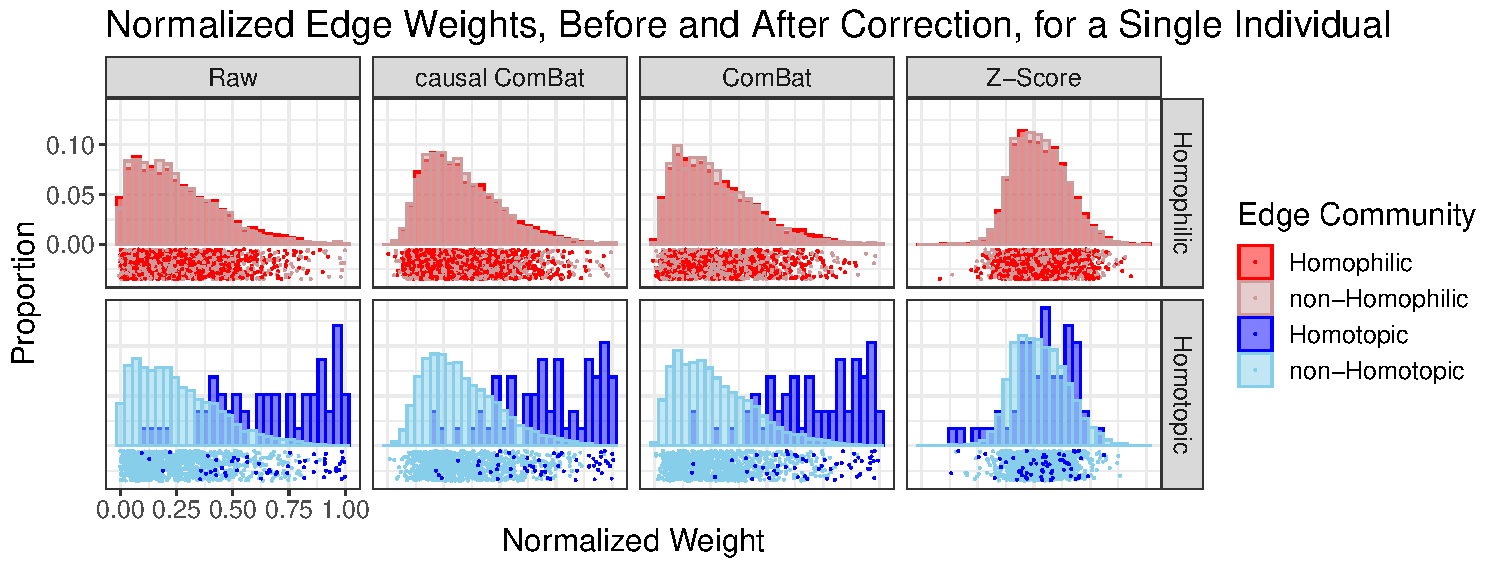
\includegraphics[width=\linewidth]{Figures/Supplement/top_hist.pdf}
    \caption{Histogram and rug plot indicating the empirical distribution of the normalized edge weights associated with each of the four edge communities for a single individual's connectome.}
    \label{fig:top_hist}
\end{figure}

Figure \ref{fig:top_hist} explores the distribution of edge weights within these two community structures before and after correction. The conclusions are similar in that Causal \Combat\ and \Combat\ preserve the property that the homotopic edges have far higher connectivity than non-homotopic edges. 